\documentclass[letterpaper]{article}
\usepackage[utf8]{inputenc}
\usepackage[parfill]{parskip}    % Activate to begin paragraphs with an empty line rather than an indent
\usepackage{graphicx}
\usepackage{amssymb}
\usepackage{amsmath}
\usepackage{amsthm}
\usepackage{mathtools}
\usepackage{mathrsfs}

\usepackage{afterpage}

\usepackage{algorithm}
\usepackage{algpseudocode}

\usepackage{verse}

\newtheorem{theorem}{Theorem}[section]
\newtheorem{corollary}{Corollary}[theorem]
\newtheorem{lemma}[theorem]{Lemma}

\theoremstyle{remark}
\newtheorem*{remark}{Remark}

\usepackage{epstopdf}
\usepackage{circuitikz}
\usetikzlibrary{angles, quotes}
\usepackage[separate-uncertainty = true,multi-part-units=single]{siunitx}
\usepackage{booktabs}
\usepackage{enumitem}
\usepackage[toc,page]{appendix}
\usepackage{color}
\usepackage{pgfplots}
\usepackage{pgfplotstable}
\usepackage{caption}
\usepackage{subcaption}
\usepackage{url}
\usepackage{multirow}
\usepackage{makecell}
\usepackage[round]{natbib}   % omit 'round' option if you prefer square brackets
\usepackage{titling}
\usepackage{siunitx}
\usepackage{physics}

\usepackage{setspace}
% \doublespacing
\usepackage{float}


\pgfplotsset{compat=1.14}

%  Special math symbols
%       floor, ceiling, angled brackets
%-----------------------------------------------------------------------
\newcommand{\floor}[1]{\left\lfloor #1\right\rfloor}
\newcommand{\ceil}[1]{\left\lceil #1\right\rceil}
\newcommand{\etal}{\textit{et al.}}
\newcommand{\RE}{\mathbb{R}}        % real space
\newcommand{\ZZ}{\mathbb{Z}}        % integers
\newcommand{\NN}{\mathbb{N}}        % natural numbers
\newcommand{\eps}{{\varepsilon}}    % prettier epsilon
%-----------------------------------------------------------------------
%  Tighter lists
%-----------------------------------------------------------------------
\newenvironment{itemize*}% Tighter itemized list
  {\begin{itemize}%
    \setlength{\itemsep}{-0.5ex}%
    \setlength{\parsep}{0pt}}%
  {\end{itemize}}
\newenvironment{description*}% Tighter description list
  {\begin{description}%
    \setlength{\itemsep}{-0.5ex}%
    \setlength{\parsep}{0pt}}%
  {\end{description}}
\newenvironment{enumerate*}% Tighter enumerated list
  {\begin{enumerate}%
    \setlength{\itemsep}{-0.5ex}%
    \setlength{\parsep}{0pt}}%
  {\end{enumerate}}
%-----------------------------------------------------------------------
% Typing shortcuts
%-----------------------------------------------------------------------
\newcommand{\X}{\mathbb{X}}
\newcommand{\SG}{\mathbf{S}}
\newcommand{\GE}{\mathcal{G}}
\newcommand{\ST}{\,:\,}
\renewcommand{\tilde}[1]{\widetilde{#1}}
\newcommand{\diam}{\mathrm{diam}}
\newcommand{\sq}{\square}
\newcommand{\half}[1]{\frac{#1}{2}}
\newcommand{\inv}[1]{\frac{1}{#1}}
\newcommand{\alg}{\textsf{SplitReduce}}
\newcommand{\sz}[1]{\sigma_{#1}}
\newcommand{\LL}{\mathcal{L}}
\newcommand{\softOmega}{\widetilde{\Omega}} 
\newcommand{\softO}{\widetilde{O}}
\newcommand{\OO}{O^*}  %or \widetilde{O}?

\newcommand{\Null}[1]{\text{Null}(#1)}


\newcommand{\dx}{\mathrm{d}x}
\newcommand{\dy}{\mathrm{d}y}
\newcommand{\dz}{\mathrm{d}z}
\newcommand{\dt}{\mathrm{d}t}
\newcommand{\du}{\mathrm{d}u}
\newcommand{\dtheta}{\mathrm{d}\theta}
\newcommand{\dq}{\mathrm{d}q}
\newcommand{\diff}{\mathrm{d}}
\newcommand{\dV}{\mathrm{d}V}
\newcommand{\dL}{\mathrm{d}L}
\newcommand{\dA}{\mathrm{d}A}
\newcommand{\dH}{\mathrm{d}H}
\newcommand{\df}{\mathrm{d}f}
\newcommand{\dg}{\mathrm{d}g}
\newcommand{\dr}{\mathrm{d}r}
\newcommand{\dw}{\mathrm{d}w}
\newcommand{\dI}{\mathrm{d}I}

\newcommand*\len[1]{\overline{#1}}


\newcommand\note[1]{\marginpar{\textcolor{red}{#1}}}
\newcommand*{\tageq}{\refstepcounter{equation}\tag{\theequation}}

\newcommand*{\equals}{=}

\usepackage{fancyhdr}

\pgfplotscreateplotcyclelist{grayscale}{
    thick,white!10!black,mark=x,mark options=solid, dashed\\%
    thick,white!20!black,mark=o,mark options=solid\\%
}

\newcommand{\mat}[1]{\ensuremath{\begin{bmatrix}#1\end{bmatrix}}}
\newcommand{\cat}[1]{\ensuremath{\begin{vmatrix}#1\end{vmatrix}}}
\newcommand{\eqn}[1]{\begin{alignat*}{4}#1\end{alignat*}}
\newcommand{\p}[2]{\frac{\partial #1}{\partial #2}}
\newcommand*{\thus}{&\implies\quad&}

\newcommand{\answer}[1]{\framebox{$\displaystyle #1 $}}

\newcommand{\shrug}[1][]{%
\begin{tikzpicture}[baseline,x=0.8\ht\strutbox,y=0.8\ht\strutbox,line width=0.125ex,#1]
\def\arm{(-2.5,0.95) to (-2,0.95) (-1.9,1) to (-1.5,0) (-1.35,0) to (-0.8,0)};
\draw \arm;
\draw[xscale=-1] \arm;
\def\headpart{(0.6,0) arc[start angle=-40, end angle=40,x radius=0.6,y radius=0.8]};
\draw \headpart;
\draw[xscale=-1] \headpart;
\def\eye{(-0.075,0.15) .. controls (0.02,0) .. (0.075,-0.15)};
\draw[shift={(-0.3,0.8)}] \eye;
\draw[shift={(0,0.85)}] \eye;
% draw mouth
\draw (-0.1,0.2) to [out=15,in=-100] (0.4,0.95); 
\end{tikzpicture}}


\pagestyle{fancy}
\fancyhf{}
\rhead{Rahul Arya}
\lhead{EE 16B}
\cfoot{\thepage}

\title{Lecture 28 - Notes}
\author{Rahul Arya}
\date{May 2019}
\begin{document}

\maketitle

\section{Overview}
Through the DFT, we have seen how arbitrary discrete-time signals can be decomposed into a sum of sinusoids. Now, we will briefly consider the continuous-time analog of that procedure, known as constructing the \emph{Fourier series} of a signal.

Specifically, we assert that for any $T$-periodic\footnote{i.e. with period $T$} scalar continuous-time signal $x(t)$, we can represent it as the infinite sum
\[
    x(t) = \sum_{l=-\infty}^\infty A_l e^{j 2 \pi l t / T},
\]
where the $A_i$ may be complex.

\section{Periodicity and nonlinearities}
First, we will look at the notion of $T$-periodicity more closely. We claim that $T$-periodicity is a property of signals that is preserved under time-invariant transformations. Specifically, if $x(t)$ is a $T$-periodic function, then for any function $f(x)$, the signal $y(t) = f(x(t))$ remains $T$-periodic.

The proof of the above result is fairly simple. By definition, a signal $x(t)$ is $T$-periodic if and only if $\hat{x}(t) = x(t + T)$ for all $t$. Thus, applying $f$ to both sides,
\eqn{
    && x(t) &= x(t + T) \\
    \thus f(x(t)) &= f(x(t + T)) \\
    \thus y(t) &= y(t + T),
}
so $y(t)$ is $T$-periodic as well, as desired.

However, it is important to recognize that, despite preserving period, nonlinear functions can still change the appearance of signals quite considerably. Consider the simple sinusoidal signal
\[
    x(t) = \sin(2\pi t)
\]
with period $T = 1$ (so it is $1$-periodic).

We will apply a nonlinear function $f(x)$ defined as follows:
\[
    f(x) = \begin{cases}
     -2 - 2x, & \text{for } {-1} \le x < -1/2 \\
     2x, & \text{for } {-1/2} \le x < 1/2 \\
     2 - 2x, & \text{for } {1/2} \le x < 1 \\
    \end{cases}.
\]
Plotting $f(x)$, we see that it looks like
\begin{center}
\begin{tikzpicture}
\begin{axis}[
    xlabel=$x$, ylabel=$ $,
    xmin=-1, xmax=1,
    ymin=-1.2, ymax=1.2,
    legend style={at={(1.02,1)},anchor=north west},
 ]
\addplot [domain=-1:-0.5, samples=100] {-2 - 2 * x};
\addplot [domain=-0.5:0.5, samples=100] {2 * x};
\addplot [domain=0.5:1, samples=100] {2 - 2 * x};
\addlegendentry{$f(x)$}
\end{axis}
\end{tikzpicture}
\end{center}

Thus, plotting both our original signal $x(t)$ and the resultant signal $y(t) = f(x(t))$ over a single period, we obtain
\begin{center}
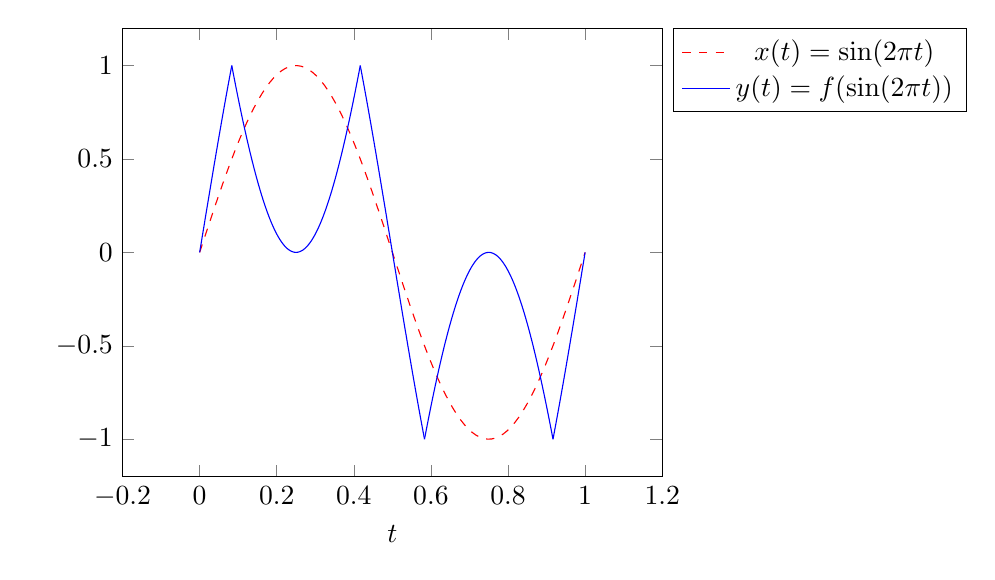
\begin{tikzpicture}
\begin{axis}[
    xlabel=$t$, ylabel=$ $,
    xmin=-0.2, xmax=1.2,
    ymin=-1.2, ymax=1.2,
    legend style={at={(1.02,1)},anchor=north west},
 ]
\addplot [domain=0:1, samples=100, red, dashed] {sin(360 * x)};
\addlegendentry{$x(t) = \sin(2\pi t)$}
\addplot [domain=0:1/12, samples=100, blue] {2 * sin(360 * x)};
\addplot [domain=1/12:5/12, samples=100, blue] {2 - 2 * sin(360 * x)};
\addplot [domain=5/12:7/12, samples=100, blue] {2 * sin(360 * x)};
\addplot [domain=7/12:11/12, samples=100, blue] {-2 - 2 * sin(360 * x)};
\addplot [domain=11/12:1, samples=100, blue] {2 * sin(360 * x)};
\addlegendentry{$y(t) = f(\sin(2\pi t))$}
\end{axis}
\end{tikzpicture}
\end{center}
Observe that $y(t)$ is radically different from $x(t)$, but still has the same period $T = 1$. In particular, notice that $y(t)$ no longer has the sinusoidal shape of $x(t)$, and that it is not differentiable everywhere.

Due to all these differences, it should therefore be surprising that we can still represent it (and ``most'' other periodic functions) as an infinite sum of sinusoids.

\section{Fourier Series}
In this course, we will not rigorously state the criteria needed for a function to equal its Fourier series, or (even for well-behaved functions) prove that the Fourier series even exists!

However, we will provide a heuristic derivation for the values of the \emph{Fourier coefficients} $A_i$ of the Fourier series of an arbitrary periodic, assuming it does exist.

Let's first write down the first few terms of the Fourier series of an arbitrary $T$-periodic function $x(t)$. For simplicity, let the fundamental frequency $f_0 = 1 / T$. Then,
\eqn{
    && x(t) &= \sum_{l=-\infty}^\infty A_l e^{j2\pi l f_0 t} \\
    &&&= A_0 + A_1 e^{j2\pi f_0 t} + A_{-1} e^{-j2\pi f_0 t} + A_2 e^{j2\pi \cdot 2 f_0 t} + A_{-2} e^{-j2\pi \cdot 2 f_0 t} + \ldots 
}
Notice that the Fourier series for a $T$-periodic function is also $T$-periodic, since all its components are harmonics of the fundamental frequency $f_0$.

Before trying to compute an arbitrary coefficient $A_l$, let's first try to solve for the DC offset $A_0$. Intuitively, each of the $e^{j2\pi l f_0}$ terms will cancel out when averaging out $x(t)$ over a full period, since their values are symmetric about the origin. Thus, after performing such an ``averaging'', we should hopefully be able to compute $A_0$.

Of course, the mathematically rigorous version of ``averaging'' is integrating, and then dividing by the period. So let's try doing just that:
\eqn{
    && \int_0^T x(t) \, \dt &= \int_0^T \sum_{l=-\infty}^\infty A_l e^{j2\pi l f_0 t} \, \dt \\
    &&&= \sum_{l=-\infty}^\infty A_l \int_0^T e^{j2\pi l f_0 t} \, \dt.
}
Now, there are two cases to consider when evaluating the integral: $l = 0$, and $l \ne 0$. When $l = 0$,
\eqn{
    && e^{j2\pi l f_0 t} &= e^{j2\pi \cdot 0 f_0 t} \\
    &&&= 1 \\
    \thus \int_0^T e^{j2\pi l f_0 t} \, \dt &= \int_0^T 1 \, \dt \\
    &&&= T,
}
and when $l \ne 0$,
\eqn{
    && \int_0^T e^{j2\pi l f_0 t} \, \dt &= \left[ \frac{1}{j2\pi l f_0} e^{j 2\pi l f_0 t} \right]_0^T \\
    &&&= \frac{1}{j2\pi l f_0} (1 - 1) \\
    &&&= 0.
}
Thus, as we expected, the sinusoidal terms all cancel out when integrated over a full period, while the DC term remains. Substituting back into our original integral, we obtain
\eqn{
    && \int_0^T x(t) \, \dt &= \sum_{l=-\infty}^\infty A_l \int_0^T e^{j2\pi l f_0 t} \, \dt \\
    &&&= A_0T + \sum_{l \ne 0} A_l \cdot 0 \\
    &&&= A_0 T.
}
Thus, we can recover the DC term
\[
    A_0 = \frac{1}{T} \int_0^T x(t) \, \dt.
\]
In other words, the DC offset of a signal is its average when integrated over a full time period, as our intuition suggested.

But what about all the other Fourier coefficients? As it turns out, this averaging trick basically still works, with a small twist. The idea is to multiply $x(t)$ with another sinusoid in order to make a particular harmonic ``look like'' the DC component. Specifically, observe that
\eqn{
    && e^{j2\pi k f_0 t} x(t) &= e^{j2\pi k f_0 t} \sum_{l=-\infty}^\infty A_l e^{j2\pi l f_0 t} \\
    &&&= \sum_{l=-\infty}^\infty A_l e^{j2\pi (l + k) f_0 t}.
}
Notice now that all the terms where $l + k \ne 0$ cancel when integrated over a full period, leaving only the $A_{-k} e^{j 2\pi (-k + k) f_0 t}$ term, letting us compute $A_{-k}$. Expressed algebraically,
\eqn{
    && \int_0^T e^{j2\pi k f_0 t} x(t) \, \dt &= A_l \sum_{l=-\infty}^\infty \int_0^T e^{j2\pi (l + k) f_0 t} \, \dt \\
    &&&= A_{-k} T,
}
since all the other integrals evaluate to $0$. Rearranging and swapping $-k$ for $k$, we find that
\[
    A_k = \frac{1}{T} \int_0^T e^{-j2\pi k f_0 t} x(t) \, \dt,
\]
allowing us to compute each of the Fourier coefficients. We can also verify that, when $k=0$, this matches our earlier result for the DC coefficient, as would be expected.

\section{Sum of Sinusoids}
Currently, the Fourier series is expressed as a sum of complex exponentials equalling a real-valued function. It would be nice to rewrite it in terms of purely real sinusoids.

Towards this end, observe that, as $x(t)$ is always real,
\eqn{
    && A_{-k} &= \frac{1}{T} \int_0^T e^{-j2\pi (-k) f_0 t} x(t) \, \dt \\
    &&&= \frac{1}{T} \int_0^T \overline{e^{-j2\pi k f_0 t}} x(t) \, \dt \\
    &&&= \overline{\frac{1}{T} \int_0^T e^{-j2\pi k f_0 t} x(t)} \, \dt \\
    &&&= \overline{A_{k}},
}
so $A_{-k}$ and $A_k$ are complex conjugates of one another. 

Now, recall that we could rearrange the Fourier series as
\eqn{
    && x(t) &= A_0 + A_1 e^{j2\pi f_0 t} + A_{-1} e^{-j2\pi f_0 t} + A_2 e^{j2\pi \cdot 2 f_0 t} + A_{-2} e^{-j2\pi \cdot 2 f_0 t} + \ldots \\
    &&&= A_0 + \sum_{l=1}^\infty A_l e^{j2\pi l f_0 t} + A_{-l} e^{-j2\pi l f_0 t}.
}
But since $A_l = \overline{A_{-l}}$, each of the terms inside the summation look a lot like the representation of sinusoids using phasors. Specifically, we have seen before that
\[
    A_l e^{j2\pi l f_0 t} + A_{-l} e^{-j2\pi l f_0 t} = M_l \cos(2\pi l f_0 t + \phi_l), 
\]
where
\eqn{
    && M_l &= 2\abs{A_l} \\
    && \phi_l &= \angle A_l.
}
Thus, we can write
\[
    x(t) = A_0 + \sum_{l=1}^\infty 2\abs{A_l} \cos(2\pi lf_0 t + \angle A_l),
\]
as a sum of sinusoids with phase shifts.

\section{Example}
Now, let's look at the Fourier series of a real periodic signal, that looks nothing like a sinusoid. The canonical example for this is the square wave with period $T = 1$, whose first period is defined piecewise as
\[
x(t) = 
\begin{cases}
     1, & \text{for } 0 \le t < 1/2 \\
     0, & \text{for } 1/2 \le t < 1 \\
\end{cases}.
\]
Using the formula for the Fourier coefficients, we find that
\eqn{
    && A_k &= \frac{1}{T} \int_0^T e^{-j2\pi k f_0 t} x(t) \, \dt \\
    &&&= \int_0^1 e^{-j2\pi k t} x(t) \, \dt.
}
We will first consider the case when $k \ne 0$. Splitting the integral up into two regions - from $0$ to $1/2$, and from $1/2$ to $1$, we find that
\eqn{
    && A_l &= \int_0^{1/2} e^{-j2\pi kt} x(t) \, \dt + \int_{1/2}^1 e^{-j2\pi kt} x(t) \, \dt \\
    &&&= \int_0^{1/2} e^{-j2\pi kt} \cdot 1 \, \dt + \int_{1/2}^1 e^{-j2\pi kt} \cdot 0 \, \dt \\
    &&&= \int_0^{1/2} e^{-j2\pi kt} \, \dt \\
    &&&= \left[\frac{1}{-j\pi k} e^{-j2\pi kt}\right]_0^{1/2} \\
    &&&= \frac{1}{-j2\pi k} \left(e^{-j\pi k t} - 1\right) \\
    &&&= \frac{1}{j2\pi k} \left(1 - e^{-j\pi k t}\right).
}

Now, we must consider the case of $k = 0$ separately, since our integration in the previous step assumed that $k \ne 0$. Rather than actually do the integral, however, we can recall that the DC coefficient $A_0$ is exactly the average of $x(t)$ over one time period, which for the case of a square wave is clearly $1/2$. Thus, we have
\[
    A_l = \begin{cases}
     1/2, & \text{if } k = 0 \\
     \frac{1}{j2\pi k} \left(1 - e^{-j\pi k t}\right), & \text{if } k \ne 0 \\
    \end{cases}.
\]

Notice that $e^{-j\pi k t}$ will alternate between $1$ and $-1$, since
\eqn{
    && e^{-j\pi 0 t} &= e^{-(0)\pi j} = 1 \\
    && e^{-j\pi 1 t} &= e^{-(1)\pi j} = -1 \\
    && e^{-j\pi 2 t} &= e^{-(2)\pi j} = 1 \\
    && \vdots
}
Thus, we have
\eqn{
    && A_0 &= 1 / 2 \\
    && A_1 &= \frac{1}{j\cdot2\pi}(1 - (-1)) = -\frac{1}{\pi}j \\
    && A_2 &= \frac{1}{2j\cdot 2\pi}(1 - 1) = 0 \\
    && A_3 &= \frac{1}{3j\cdot 2\pi}(1 - (-1)) = -\frac{1}{3\pi}j \\
    && \vdots
}

In other words,
\[
A_l = \begin{cases}
     \frac{1}{2}, & \text{if } k = 0 \\
     0, & \text{if } k \ne 0 \text{ and is even} \\
     -\frac{1}{k\pi} j, & \text{if } k \ne 0 \text{ and is odd} \\
    \end{cases}.
\]

Now, observe that
\[
\abs{A_l} = \begin{cases}
     \frac{1}{2}, & \text{if } k = 0 \\
     0, & \text{if } k \ne 0 \text{ and is even} \\
     \frac{1}{k\pi}, & \text{if } k \ne 0 \text{ and is odd} \\
    \end{cases}.
\]
and
\[
\angle{A_l} = \begin{cases}
     0, & \text{if } k = 0 \\
     \text{undefined}, & \text{if } k \ne 0 \text{ and is even} \\
     3\pi/2, & \text{if } k \ne 0 \text{ and is odd} \\
    \end{cases}.
\]

As a consequence, using our result from the previous section, we can express $x(t)$ as the summation
\eqn{
    && x(t) &= A_0 + \sum_{l=1}^\infty 2\abs{A_l} \cos(2\pi lf_0 t + \angle A_l) \\
    &&&= \frac{1}{2} + \frac{2}{\pi} \cos(2\pi t + 3\pi/2) + \frac{2}{3\pi} \cos(2\pi \cdot 3 t + 3\pi/2) + \ldots \\
    &&&= \frac{1}{2} + \frac{2}{\pi} \sin(2\pi t) + \frac{2}{3\pi} \sin(2\pi \cdot 3 t) + \ldots
}

Plotting the first five terms of the above summation over a single period, we obtain
\begin{center}
\begin{tikzpicture}
\begin{axis}[
    xlabel=$t$, ylabel=$ $,
    xmin=-0.2, xmax=1.2,
    ymin=-0.2, ymax=1.2,
    legend style={at={(1.02,1)},anchor=north west},
 ]
\addplot [domain=0:0.5, samples=100, red, forget plot] {1};
\addplot [domain=0.5:1, samples=100, red] {0};
\addlegendentry{$x(t)$}
\addplot [domain=0:1, samples=100, blue] {1/2 + 2 / pi * sin(360 * x) + 2 / (3 * pi) * sin(360 * 3 * x) + 2 / (5 * pi) * sin(360 * 5 * x) + 2 / (7 * pi) * sin(360 * 7 * x)};
\addlegendentry{Truncated Fourier approximation to $x(t)$}
\end{axis}
\end{tikzpicture}
\end{center}
indicating that even just a few terms of the Fourier series form a pretty good approximation to our function!

Notice, however, that the error is largest near the beginning and end of the period, as well as near the central discontinuity of the square wave. By considering more terms, this effect becomes more pronounced. With $10$ terms, we obtain
\begin{center}
\begin{tikzpicture}
\begin{axis}[
    xlabel=$t$, ylabel=$ $,
    xmin=-0.2, xmax=1.2,
    ymin=-0.2, ymax=1.2,
    legend style={at={(1.02,1)},anchor=north west},
 ]
\addplot [domain=0:0.5, samples=100, red, forget plot] {1};
\addplot [domain=0.5:1, samples=100, red] {0};
\addlegendentry{$x(t)$}
\addplot [domain=0:1, samples=100, blue] {1/2 + 2 / pi * sin(360 * x) + 2 / (3 * pi) * sin(360 * 3 * x) + 2 / (5 * pi) * sin(360 * 5 * x) + 2 / (7 * pi) * sin(360 * 7 * x) + 2 / (9 * pi) * sin(360 * 9 * x) + 2 / (11 * pi) * sin(360 * 11 * x) + 2 / (13 * pi) * sin(360 * 13 * x) + 2 / (15 * pi) * sin(360 * 15 * x) + 2 / (17 * pi) * sin(360 * 17 * x)};
\addlegendentry{Truncated Fourier approximation to $x(t)$}
\end{axis}
\end{tikzpicture}
\end{center}
Notice that the spikes near the discontinuities have become much more significant. This may remind you of Runge's phenomenon in polynomial interpolation, and is indeed a very similar effect, known as the \emph{Gibbs phenomenon}. 

Although we will not discuss it in great detail, it is interesting to know that no matter how many terms of the Fourier series we evaluate, there will always be an error near the discontinuities of our true signal. Intuitively, we can justify this by arguing that we are attempting to approximate a discontinuous function with an infinite series of smooth functions, which will inevitably lead to some error.

\section{Truncated Fourier Series}
Notice in the previous section that even the first $5$ or $10$ terms of the Fourier series offered a fairly decent approximation to the true function for most values of $t$. Furthermore, the truncated Fourier series seemed to converge on its limiting value fairly rapidly as more terms were added, though this limiting value still did not equal the original function at all points.

A natural question that arises is as follows: does the Fourier series always converge? As it turns out, the answer is yes! Specifically, for any given value of $\eps$, there exists a (finite) $m$ such that the error function
\[
    \abs{\sum_{l=-m}^m A_l e^{j2\pi f_0 l t} - \sum_{l=-\infty}^\infty A_l e^{j2\pi f_0 l t}}
\]
is bounded by $\eps$ for all value of $t$. That is to say, we can get a truncated Fourier series arbitrarily close to the limiting value by simply including enough terms.

While we will not prove this result mathematically, we will provide some physical intuition as justification. In the real world, signals are generated by some physical process. Currently, the frequencies used in electronics are bounded by $10^{18}\SI{}{\hertz}$ due to physical processes. In practice, it is unlikely that we will exceed $10^{15}\SI{}{\hertz}$ in the near future. Even in nature, we rarely see frequencies greater than about $10^{25} \SI{}{\hertz}$. Thus, by truncating our Fourier series after that point, we can be confident that we have produced a good approximation for our observed signal. And in practice, we can typically truncate our series with far fewer terms, say around $10^{10}$ at the most.

\section{Wrapping Up}
That's it! We're done! Hope these notes were useful. Have fun with the final. Here's a cat:
\begin{center}
\includegraphics[width=0.8\textwidth]{lecture_28/cat.jpg}
\end{center}

\end{document}
